\clearpage
\VerdierPhysicalPageAnchor{0089}%
\VerdierSemanticAnchor{ch1-3-2-5-composite-zero-conclusion}
したがってこれは零である。よって、写像錐関手の随伴性 (3.1.3) により、
一意な射

\VerdierSemanticAnchor{ch1-3-2-5-eq2}
\begin{equation}
  J\colon c(p(f))\longrightarrow X[1]
  \tag{3.2.5.2}
\end{equation}

\noindent が存在し、次の図式が可換となる：

\VerdierSemanticAnchor{ch1-3-2-5-eq3}
\VerdierSemanticAnchor{ch1-3-2-5-j-comparison-diagram}
\begin{equation}
  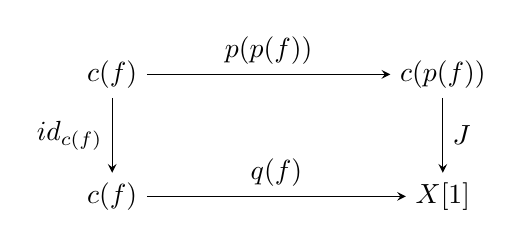
\begin{tikzpicture}[>=stealth,baseline=(current bounding box.center)]
    \node (Cf1) at (0,1.55) {$c(f)$};
    \node (Cpf) at (4.2,1.55) {$c(p(f))$};
    \node (Cf2) at (0,0) {$c(f)$};
    \node (Xs)  at (4.2,0) {$X[1]$};
    \draw[->] (Cf1) -- node[above] {$p(p(f))$} (Cpf);
    \draw[->] (Cf1) -- node[left] {$\operatorname{id}_{c(f)}$} (Cf2);
    \draw[->] (Cpf) -- node[right] {$J$} (Xs);
    \draw[->] (Cf2) -- node[above] {$q(f)$} (Xs);
  \end{tikzpicture}
  \tag{3.2.5.3}
\end{equation}

\noindent さらに $Ja(p(f))=0$ (3.1.2.4) である。

\VerdierSemanticAnchor{ch1-3-2-6}
\noindent\textbf{命題 3.2.6.}\quad
\VerdierSemanticAnchor{ch1-3-2-6-a}
\emph{a) 射 $J$ はホモトピー同値、すなわちホモトピーを除いて同型である。}

\VerdierSemanticAnchor{ch1-3-2-6-b}
\emph{b) 次の図式}

\VerdierSemanticAnchor{ch1-3-2-6-eq1}
\begin{equation}
  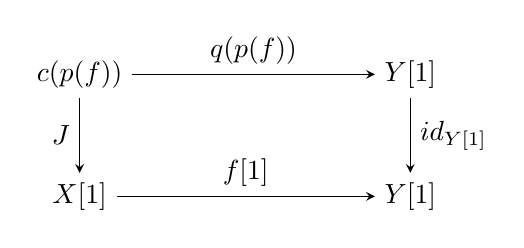
\begin{tikzpicture}[>=stealth,baseline=(current bounding box.center)]
    \node (Cpf) at (0,1.55) {$c(p(f))$};
    \node (Ys1) at (4.2,1.55) {$Y[1]$};
    \node (Xs)  at (0,0) {$X[1]$};
    \node (Ys2) at (4.2,0) {$Y[1]$};
    \draw[->] (Cpf) -- node[above] {$q(p(f))$} (Ys1);
    \draw[->] (Cpf) -- node[left] {$J$} (Xs);
    \draw[->] (Ys1) -- node[right] {$\operatorname{id}_{Y[1]}$} (Ys2);
    \draw[->] (Xs) -- node[above] {$f[1]$} (Ys2);
  \end{tikzpicture}
  \tag{3.2.6.1}
\end{equation}

\noindent\emph{はホモトピーを除いて反可換である。}

\VerdierSemanticAnchor{ch1-3-2-7}
\noindent\textbf{3.2.7. 証明。}\quad
\VerdierSemanticAnchor{ch1-3-2-7-h-construction}
まず射 $H\colon X[1]\longrightarrow c(p(f))$ を構成する。
\VerdierSemanticAnchor{ch1-3-2-7-representing-functors}
そのためには、この二つの対象が表現する二つの関手の間の射を構成すればよい。
$W$ を $\operatorname{comp}(C)$ の対象とする。
\VerdierSemanticAnchor{ch1-3-2-7-pair}
写像錐関手の随伴性 (3.1.3) を考慮すれば、$c(p(f))$ から $W$ への射とは、
$u\colon c(f)\longrightarrow W$ が複体の射で、
$a\colon0\rightsquigarrow up(f)$ がホモトピーであるような組 $(u,a)$ に
ほかならない。
\VerdierSemanticAnchor{ch1-3-2-7-triple}
再び (3.1.3) を用いると、$c(p(f))$ から $W$ への射は三つ組
\begin{equation*}
  \bigl(m\colon Y\longrightarrow W,\quad
  a\colon0\rightsquigarrow m,\quad
  b\colon0\rightsquigarrow mf\bigr)
\end{equation*}
であることがわかる。この三つ組に次の図式を対応させる：

\VerdierSemanticAnchor{ch1-3-2-7-eq1}
\begin{equation}
  \begin{gathered}
    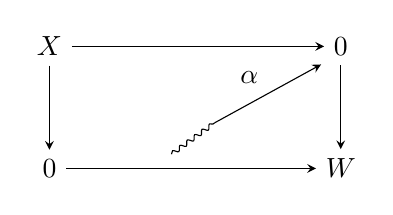
\begin{tikzpicture}[>=stealth,baseline=(current bounding box.center)]
      \node (X)  at (0,1.55) {$X$};
      \node (Z1) at (3.7,1.55) {$0$};
      \node (Z2) at (0,0) {$0$};
      \node (W)  at (3.7,0) {$W$};
      \draw[->] (X) -- (Z1);
      \draw[->] (X) -- (Z2);
      \draw[->] (Z1) -- (W);
      \draw[->] (Z2) -- (W);
      \draw[decorate,decoration={snake,amplitude=0.8pt,segment length=3.3pt}]
        (1.55,0.18) -- (2.10,0.58);
      \draw[->] (2.10,0.58) -- node[above left] {$\alpha$} (3.45,1.32);
    \end{tikzpicture}
    \qquad \alpha=b-a\star f ,
  \end{gathered}
  \tag{3.2.7.1}
\end{equation}
